 %%%%%%%%%%%%%%%%%%%%%%%%%%%%%%%%%%%%%%%%%
% Academic Title Page
% LaTeX Template
% Version 2.0 (17/7/17)
%
% This template was downloaded from:
% http://www.LaTeXTemplates.com
%
% Original author:
% WikiBooks (LaTeX - Title Creation) with modifications by:
% Vel (vel@latextemplates.com)
%
% License:
% CC BY-NC-SA 3.0 (http://creativecommons.org/licenses/by-nc-sa/3.0/)
% 
% Instructions for using this template:
% This title page is capable of being compiled as is. This is not useful for 
% including it in another document. To do this, you have two options: 
%
% 1) Copy/paste everything between \begin{document} and \end{document} 
% starting at \begin{titlepage} and paste this into another LaTeX file where you 
% want your title page.
% OR
% 2) Remove everything outside the \begin{titlepage} and \end{titlepage}, rename
% this file and move it to the same directory as the LaTeX file you wish to add it to. 
% Then add \input{./<new filename>.tex} to your LaTeX file where you want your
% title page.
%
%%%%%%%%%%%%%%%%%%%%%%%%%%%%%%%%%%%%%%%%%

%----------------------------------------------------------------------------------------
%	PACKAGES AND OTHER DOCUMENT CONFIGURATIONS
%----------------------------------------------------------------------------------------

\documentclass[10pt]{article}

\usepackage[utf8]{inputenc} % Required for inputting international characters
\usepackage[T1]{fontenc} % Output font encoding for international characters
\usepackage{mathpazo} % Palatino font
\usepackage{tocloft,lipsum,pgffor,sectsty}
 \usepackage{url, longtable}

\setcounter{tocdepth}{3}% Include up to \subsubsection in ToC

% Font changes to ToC content of sectional units
\renewcommand{\cftsecfont}{\LARGE\scshape}
\renewcommand{\cftpartfont}{\normalfont\sffamily\bfseries}% \part font in ToC
\renewcommand{\cftsecfont}{\normalfont\slshape}           % \section font in ToC
\renewcommand{\cftsubsecfont}{\normalfont\itshape}        % \subsection font in ToC
\renewcommand{\cftsubsubsecfont}{\normalfont\small}       % \subsubsection font in ToC

% Font changes to document content of sectional units
\renewcommand{\partfont}{\normalfont\Huge\bfseries}
\renewcommand{\chapterfont}{\normalfont\huge\bfseries}
\renewcommand{\sectionfont}{\normalfont\LARGE\bfseries}

\usepackage{graphicx}
\graphicspath{ {images/} }


\begin{document}

%----------------------------------------------------------------------------------------
%	TITLE PAGE
%----------------------------------------------------------------------------------------

\begin{titlepage} % Suppresses displaying the page number on the title page and the subsequent page counts as page 1
	\newcommand{\HRule}{\rule{\linewidth}{0.5mm}} % Defines a new command for horizontal lines, change thickness here
	
	\center % Centre everything on the page
	
	%------------------------------------------------
	%	Headings
	%------------------------------------------------
	
	\textsc{\LARGE INF-3910-3-3 - Computer Science Seminar: IoT services with LoRaWAN network and compatible embedded devices and sensors}\\[1.5cm] % Main heading such as the name of your university/college
	
	\textsc{\Large University of Tromsø}\\[0.5cm] % Major heading such as course name
	
	
	%------------------------------------------------
	%	Title
	%------------------------------------------------
	
	
	
	{\huge\bfseries Animal tracker project }\\[0.4cm] % Title of your document

	%------------------------------------------------
	%	Author(s)
	%------------------------------------------------
	
	% If you don't want a supervisor, uncomment the two lines below and comment the code above
	{\Large{Thomas Bye Nilsen\\Valter Berg}}
	%------------------------------------------------
	%	Date
	%------------------------------------------------
	
	\vfill\vfill\vfill % Position the date 3/4 down the remaining page
	
	{\large\today} % Date, change the \today to a set date if you want to be precise
		
	\vfill % Push the date up 1/4 of the remaining page
	
\end{titlepage}

\tableofcontents
\listoffigures
%\listoftables

\clearpage

\section{Introduction}
	This report describes the work that lays the foundation for our project. The project is about tracking certain animals in their natural habitat without hindering their way of living. The motivation for our project is the usefulness of the services provided by the system we develop. Animal keepers can track down and survey individuals as they are in movement in their natural habitat.

	\subsection{Problem statement}
		The problem we want to solve is to gather and present data regarding the environment and movement patterns of the animals using IoT devices. We want to make the IoT devices fit as many species as possible. We will track animals by emitting GPS coordinates, accelerometer data, battery voltage and temperature from the IoT devices. All data will be delivered to a front-end system through the LoRaWAN network. 
		\\\\
		We will primarily focus on gathering the four attributes from an arbitrary number of observational units; we will not focus on creating a mesh network of IoT devices. 
		\\\\
		The complexity of the project is not too high for a practical completion. The technology needed is available and there seems to be not too much work to achieve it. After one week we will design the architecture of the system and make a list of equipment we need. We expect that we will acquire enough low-level details of the technical requirements after a few weeks to implement most of the core functionalities by milestone 3. The remaining functionalities will be postponed to milestone 4, if any. Soldering of electronics will take about one day. Designing and printing the box will take about one day as well. Designing and implementing the front-end system will take between one and two weeks. Bridging the transmission between the different components in system will take a few days. The time estimates include testing and debugging. 
		\\\\
		In addition, we have been in contact with Rovdata, a company that tracks wild animals for the purpose of population control and positional tracking. We also contacted some farmers who work with sheep herding to see if they could contribute with any opinions on the concept and design. The farmers were positive to our design and concept, but they were concerned about the total cost of implementing such a system on all their sheep, as they have 300 to 600 individuals grassing each summer. That is why we also intend to keep the cost as low as possible, which also should be an advantage with using cheap LoPy devices and a low-cost network such as LoRa. 


	\subsection{Background}
		\textbf{Hardware} \\
		For the processing device we use a Lopy, a MicroPython enabled microcontroller, with LoRa connectivity as one of its features.  The LoPy is mounted on a Pytrack extension board which provide a GNSS and Glonass GPS system, and a three axis accelerometer.  The temperature sensor is a DS18B20 one-wire digital temperature sensor. It reports degrees in Celsius in the range -55C to 125C (+/-0.5C)\cite{tempsensor}. Figure 1 displays the data sheet for a Pytrack and figure 2 displays the data sheet for DS18B20.
		\\
		\begin{figure}[h]
			\caption{Pytrack data sheet}
			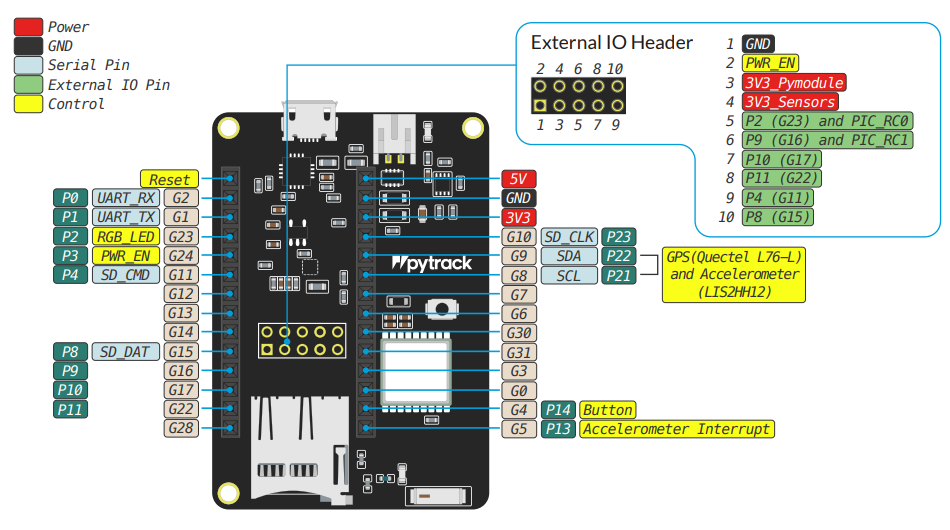
\includegraphics[width=10cm, height=6cm]{pytrackdatasheet}
		\end{figure}
		
		\begin{figure}[h]
			\caption{DS18B20 data sheet}
			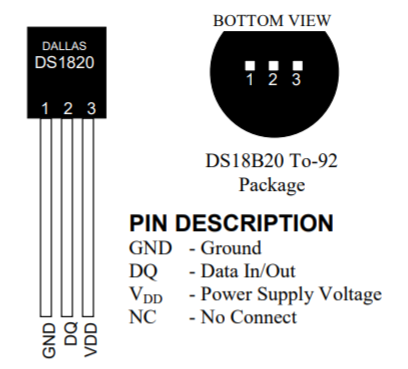
\includegraphics[width=6cm, height=6cm]{tempsensordatasheet}
		\end{figure}
\textbf{LoRaWAN}
		LoRaWAN is a long range wide area network protocol designed to wirelessly connect small battery powered devices to the internet. It targets important internet of things features such as bi-directional communication, end-to-end security and mobility. LoRaWAN fits in the second and third layer of the OSI model, implemented on top of LoRa or FSK modulation in industrial, scientific and medical radio bands\cite{LoRaWAN}.
		\\\\
		\textbf{Mqtt and Managed IoT Cloud} \\
		MQTT, or Message Queue Telemetry Transport, is a machine to machine/internet of things connectivity protocol based on publish-subscribe messaging. This protocol works on top of the TCP/IP protocols and enables communication with remote locations where small footprints are required or the bandwidth is limited. To do the publish-subscribe messaging, there is a message broker which distributes messages to connected clients based on the topic of the message\cite{wikiMQTT}. The Managed Iot Cloud (MIC), provided by Telenor, uses MQTT as its main protocol in the underlying AWS Iot Message broker for thing-to-backend communication. The Managed IoT Cloud platform enables managing of the IoT broker and data is routed through exposed MQTT topics. The MIC cloud platforms provides a user interface to view reported date from Lopy and gives you the opportunity to format the data sent to the Mqtt broker\cite{telenorIOT}.
		
		
		
	\subsection{Member roles}
		The team members are Valter Berg and Thomas Bye Nilsen. The member agree on the tasks that are to be solved. Below is a table of features that we will be working on and who will be working on it. For some features, mainly in the beginning of the project, both members conduct. This approach seems convenient to give both members a better understanding of the technical details, e.g how to emit simple GPS data from lopy device to IoT cloud. Both members will update each other on the state of the feature they work on and provide each other with input. 
		\\\\
		\begin{longtable}{ | p{10cm} | p{1.3cm}|}
			\hline
			\textbf{Feature} & \textbf{Member}\\ \hline
			Contact farmers & Valter\\ \hline
			Contact Rovdata & Thomas\\ \hline
			Test GPS and accelerometer, write basic script code for LoPy & Both\\ \hline
			Solder temperature sensor, write test code, perform testing & Thomas\\ \hline
			Solder battery package & Thomas\\ \hline
			Design and print box. Test it in realistic envrionment & Thomas\\ \hline
			Research front-end API and framework & Both\\ \hline
			Login on front-end. Research database system for users & Thomas\\ \hline
			Design login view & Valter\\ \hline
			Setup remote database for users & Valter\\ \hline
			Query historic data and prepare data for view on a map & Thomas\\ \hline
			Find map provider and write API for displaying positions & Valter\\ \hline
			Write server code for MQTT connection and live updates from Telenor Managed IoT Cloud and listen on all devices & Valter\\ \hline
			Make front-end view for live or last update, toggle option for previous positions& Valter\\ \hline
			Make GUI and back-end functionalities to edit properties with Telenor Cloud API. Simple GUI to edit update rate and save changes in a database & Valter\\ \hline
			Implement fault-tolerance and deep sleep on Lopy, perform tests & Valter\\ \hline
			Setup server instance at Heroku for hosting & Valter\\ \hline
			Test features and system behvaiour(e.g. battery life, signal strengths) & Both\\ \hline
			Measure power consumption in deep sleep and work mode & Thomas\\ \hline
			Generate dummy sensor data with script, used for testing of server and front-end & Valter\\ \hline
		\end{longtable}
		The rest of the report is laid out as milestone chapters, starting from milestone 2. The milestones are laid out on a timeline that incrementally build a solution to the problem. Milestone 2 includes the project design, a high-level priority list of features to implement, technical design and outlining of risks, as well as how they will be mitigated. Milestone 3 describes the state of the project after implementing the core functionalities and the path to achieve it, as well as any observations made. Milestone 4 describes the remaining implementation choices, the path the project took from milestone 3 and end-state of the project. Finally, there will be an analysis of some of the aspects in the project. At last, we will draw a conclusion. 		
		

\section{Milestone 2}
	\subsection{Design decisions}
		As of 19th of February, all design decisions are clarified. To gather relevant data, we learn that two Pytrack expansion boards and two temperature sensor are suitable for our use because they provide all the features we need. The relevant components are one GPS transmitter, accelerometer sensor and a DS18B20 one-wire digital temperature sensor on each board. The GPS transmitter and the accelerometer sensor are embedded in the Pytrack. We need to focus on the power consumption because animals are in their natural habitat for months at a time, depending on the species. We would like to make the sensors as low-powered as possible because it takes time to replace the battery packages. Because of the LoRaWAN’s bandwidth limitations and battery life limitation, we need to pay attention to the size of the data that are sent. We also need to focus on the design of the boxes. An important aspect is that they must not bother the animals. In addition, it must be waterproof and able to withstand nudges and that they don't fall off the wearer. Finally, we need to securely present the data that are meaningful and intuitive to the end-user.
		\\\\
		We prioritize the order in which the features are implemented. The features that must be included are:
		\begin{itemize}  
			\item Gather GPS coordinates, accelerometer data, battery voltage and temperature readings on the senors
			\item Send the gathered data to a MIC Cloud instance provided by Telenor
			\item Send data from MIC Cloud to a front-end system
			\item Implement a front-end system with login sessions
			\item Show the GPS coordinates in a map, along with time stamps and temperature readings
		\end{itemize}
		These requirements are needed to make up a minimal standard for the project's result. 
		\\\\
		The features that should be included:
		\begin{itemize}  
			\item Two-way communication with MQTT, being able to change state at lopy, e.g. update rate. 
			\item Show info and previous positions for each device
			\item Upon no movement registered with gps, or lack of gps signal, automatically use accelerometer to verify that the animal is still alive and moving. Give notification in GUI of result. 
			\item Notify if some individuals are in unwanted positions, such as close to village, roads or similar places.
			
		\end{itemize}
		The features that could be included are:
		\begin{itemize}  
			\item Notify subscribed users on email or phone if interesting events happen
			\item Implement a smart phone application that interfaces with the system
			\item Comprehensive info about each animal.
			\item Show any grassing areas that are beneficial to weight conditions or other factors
		\end{itemize}
		
		The feature that we will not include is 
		\begin{itemize}
			\item Direct communication between the observational units
		\end{itemize}

	\subsection{Overall flow and states}
		So far we have a direction and goal for the project. We have a list for all the sensors we need, an architecture for the system and we also know how to design boxes that will be 3D-printed. In addition, we have setup a development environment and tested the LoPy device by sending some arbitrary data to MIC Cloud. We have also looked into popular development frameworks for implementing a back-end system for presenting the data.
	
	\subsection{Estimated time for work}
		Taking the current state of the project into consideration, we believe we are on schedule. By the time of milestone 3, we aim to have implemented most of the features on the server and on the observational units. We think that between milestone 3 and milestone 4 we implement all the remaining features. 
		
	\subsection{Technical design}
		We begin by describing the architecture of the system, the choices made and why they were made. The architecture is visualized in figure 3. 
		
		\begin{figure}[h]
			\caption{Architecture}
			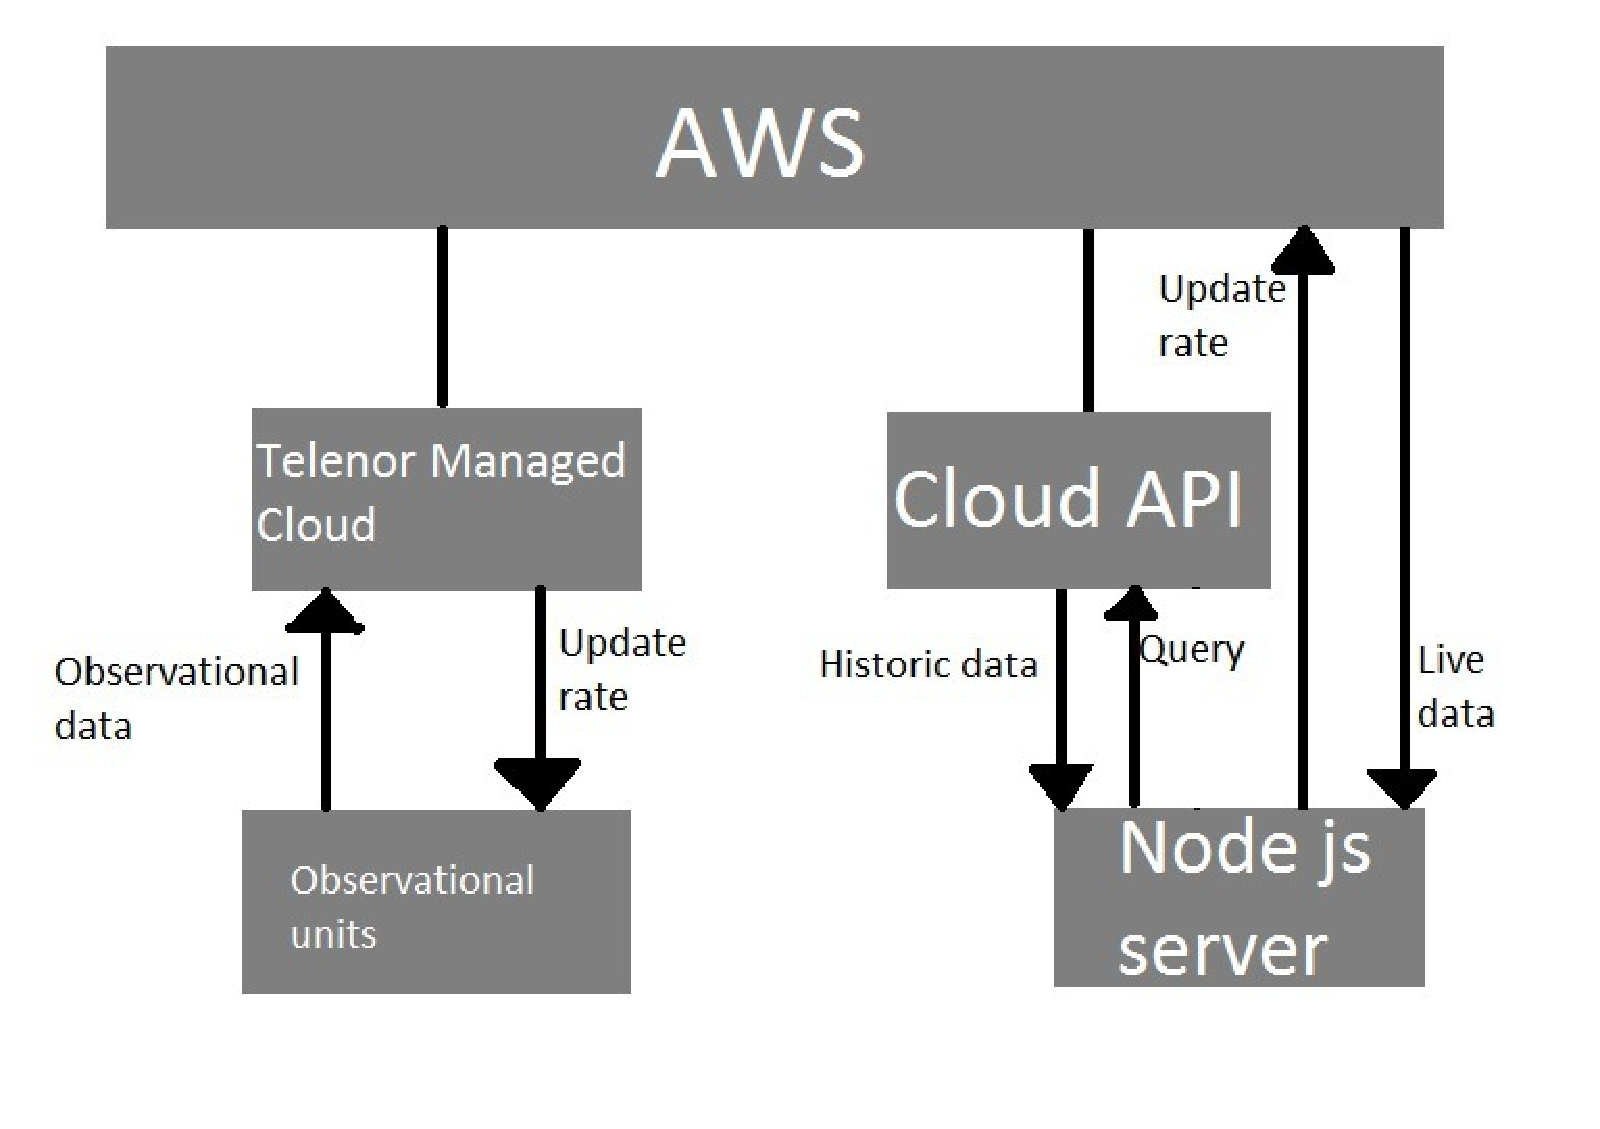
\includegraphics[width=10cm, height=6cm]{images/architecture.pdf}
		\end{figure}

		This is a distributed system with observational units on the edge, a cloud instance and a server with a front-end system. The AWS box in the figure is both the message broker for Mqtt transactions and were thing properties and historic data is stored in buckets. The MIC cloud handles LoRa connection with the Lopy devices and publishes formated data on a specific topic to the Mqtt broker at AWS. The node js server subscribes on the topic for the observation data from the AWS broker. The observation data is stored in buckets at AWS and are reached through a cloud API provided by telenor. The cloud API is also used for updating thing properties such as name and descriptions. The node js server also interact with a MongoDb database, although it is only used for login credentials and other small properties concerning our website(Not in the figure) . 
		\\\\
		There is an arbitrary number of homogeneous observational units on the edge, each of which gathers data. Their homogeneity comes from the fact that they perform the same tasks in the same order. However, they might do their tasks at different points in time. Each observational unit will gather temperature in Celsius, GPS coordinates, accelerometer data and battery voltage. They will regularly send the observational data to the Telenor MIC Cloud using the LoRaWAN protocol. The data is transmitted over LoRa network because it is important to have long range connections and low power consumption. It is also within the scope of the assignment to use LoRaWAN to connect with the Lopy devices.  
		\\\\
		We need a server with a front-end that displays the data because we can fine-tune the presentation of the data. It can also be more user-friendly than the provided MIC cloud GUI from Telenor. In addition, we would like to emulate a real-world user’s point of view from this front-end system. To enforce security measurements on the front-end component, we want a login feature. We want to make it possible for the end-user to manage the sensors from the front-end. This feature simplifies the process of naming sensors and managing their properties. 	
		\\\\
		We need to show the positions in a map because knowing the position of the devices is the essential of this project. For each data point in the time interval $T_1$ to $T_2$, the longitude coordinate, latitude coordinate, temperature and battery voltage are displayed. The time is given in the ISO date. The longitude and latitude coordinates are marked on a two-dimensional map as a single point. The temperature, accelerometer and battery are also displayed at given points in time. This is so the user can access vital information on the current state of each device, specially upon abnormal events. These abnormal events can be too low temperatures where an animal keeper may want to track down the individuals and possibly move the pack. Also, researchers can look at the relation between geographical areas in which individuals are located and the temperatures in the areas. The battery voltage is needed so that an observational unit is able to alert the end-user of low battery life.  	
		\\\\
		The accelerometer data is used as a indicator along with the GPS data to see if a individual is likely to be deceased. If an individual has not changed its GPS position, it should be possible to see if the accelerometer data within a given time frame has changed. It may strengthen or weaken the suspicion of a deceased individual. If there is no GPS signal, the other observational data points are still sent. The accelerometer data can indicate whether or not an individual is still alive even though there is no GPS coverage.The time frame has yet to be decided through parameter adjustments. Because it is possible that the IoT device sends data at the time an individual sleeps, the time frame must be adjusted. For example, if an observational unit transmits data once a night, the animal might be at rest at a 
		position it favours. The animal is still alive, but the sensor readings tell that it has not moved. However, if the update rate is rapidly (e.g. once every tenth minute) and the GPS coordinates and the accelerometer data don’t change over some period of time, it is likely that the animal is deceased. This should be recognized by the system itself, either server side or at the device, and then perform tests with increasing the update rate for reading sensor data. The state should then be presented with an alert level according to the adversity of the results.
		\\\\
		A two-way communication is needed so that the end-user is able to adjust the rate at which a particular observational unit sends data. The update rate should be multi-casted; a broadcast is not needed because there might be situation where only one individual needs to be tracked down with higher update rate. However, a broadcast is possible by toggling how many observational units that are to be updated. A situation where two-way communication is needed is  when a wolf is in its natural habitat the update rate can be as low as one transmit per day. When the same wolf is to be tracked down for research purposes, the end-user can increase the update rate to several times per minute. This feature enables the end-user to prolong the battery life to the fullest extent. This feature makes the system more agile with respect to battery life. A two-way communication is also needed when checking a suspicion of a deceased animal server side, where the server might have to adjust the interval of the device emit rate. 

\section{Milestone 3}
	As of 19th of March, we have implemented most of the core functionalities on the edge and the front-end. We have made progress on all components of the system. The equipments that we use are two Pytrack expansion boards and two DS18B20 one-wire temperature sensors. From the technical specifications drafted in milestone 2, we have decided for most of the low-level details. An important point to make is that observational data is transferred from the edge to the front-end system. We have made several discoveries since previous milestone that need to be addressed.
 

	\subsection{Sensor side}
		We have managed to gather GPS data and battery voltage from one of the two observational units. We have yet to implement the features on both Pytrack boards. In the development phase, we choose to omit one Pytrack board because their hardware components are homogeneous. It is fairly simple to upload the code used on one of the boards to the other board. We implement the Pytrack boards using MicroPython. We successfully send the gathered data with LoRaWAN to a Managed IoT Cloud instance. We use a 3.7V battery 600 mAh battery to power the sensor. When we deploy the sensor in a real-world environment in lower temperatures, we will use a bigger battery. \\\\
		 We have also been looking at accelerometer data readings. We observe that the accelerometer values fluctuate in all three dimensions by about +/- 0.001g, even when the accelerometer is standing completely still. We think we can introduce an interval between which the values can fluctuate so that the system can ignore negligible fluctuations. Since we are interested in any movement regardless of its direction, the values for movement in x, y and z direction is summed together before they are sent. The summation of the data is reduced to three significant figures, as a more accurate precision is useless because of the fluctuation in the values. This also reduces the data size that has to be emitted. 
		 \\\\
		 The format of the data that we send is <longitude, latitude, battery voltage, temperature, accelerometer>. As of now, we only generate data for temperature since the actual sensor is still to be mounted on the Lopy device. The size of the payload we send is either 24 bytes or 34 bytes.The size depends on whether or not there is GPS coverage in the area. The values in the payload are separated by whitespaces. If there isn’t GPS coverage, we choose to send empty default values for longitude and latitude coordinates.
		\\\\
		We choose still to send temperature readings and battery voltage if there is no GPS coverage because the data being sent are still useful. For example, if a sheep wears the observational unit and the end-user sees that the temperature drops to very low temperatures, the end-user can still take actions. The limitation, however, is the fact that the end-user is not aware of the sheep’s location. The battery voltage reading still serves its purpose of telling how long the observational unit has to live.
		
	\subsection{Telenor MIC Cloud}
		We read observational data on Telenor MIC Cloud by specifying the format of the observational data received from the Lopy. We successfully visualize the received data with the MIC cloud GUI widgets. This is very useful when testing the devices on connection and content of the data. Sending the data to the observational units is still an open issue.
	 
		
	\subsection{Front-end}
		We have implemented a website with html, css and javascript for front-end and using the Node JS server environment for back-end. We are somewhat familiar with Node JS and we know it has suitable packages since it is used in all the tutorials about MQTT connection and cloud API.  To display map we use the open source library Leaflet which provide a user friendly interface to display maps. We use maps from NorgesKart because it provides a detailed and much descriptive map of Norway at no cost. It is especially useful for displaying points, given longitude and latitude coordinates, which is what we need. We are able to subscribe on topics at the Mwtt broker at AWS and receives the published observational data from the Lopys. We also do queries for older observation data with use of the cloud api and display things positions on the map. 
		\\\\
		We made feature for editing things in the Managed IoT Cloud with use of the Cloud API. This feature provides possibility to edit the thing name and description in the frontend website. This feature is implemented since it is likely that it is more convenient to have other information on a animal then just an ID nummer. For example you could note number of lambs for a sheep, weights or other info about a individ that could be useful to know. This info should then be connected with thigns shown on the map in an intuitive way. As of now they can be viewed in the editing table.  
		\\\\
		We choose to protect the front-end with password authentication because we believe that security is an important aspect of this project. Although the project is not planned to be shipped into production, it is worth applying best practices. After authentication, the user manages the front-end as it sees fit.
		\\\\
		To test the front-end and its behavior with more data and units, we wrote a script for dummy units publishing generated observational data to the Mqtt broker.   
		
\section{Milestone 4}
	As of 18th of April we have made progress on several aspects of the project. We have refined some of our approaches on the features since milestone 3 and implemented some new features as well. 
	\subsection{Sensor side}
		There is now implemented deep-sleep at the Lopy where the sleep time is set static in the code. The deep-sleep is initiated when the all the sensor data is read and sent further over the LoRa connection. When the device awakes from the sleep it should fetch and send sensor data, before it falls into deep-sleep again. Therefore the sleep time will decide the interval on the rate that observational data is transmitted and is the value that should be set when changing the update rate. The decision to use deep-sleep is made upon the interest of reducing power consumption by reducing the processing time for the unit. There occurred some challenges since the device reboots after each time it awakes meaning that the previous state of the device is forgotten. This includes the already established connection with LoRa, which made the device use a significant time on reestablishing the connection on each awakening. To reduce the processing time, the established connection is saved to a none-volatile memory on the unit where it is read from upon a awakening. To check if a connection is stored, a validation number is also saved each time an connection successfully is established. The decision of saving the connection was made since it is in our interest to reduce the processing time and power consumption. The effects on the battery lifetime with implementing deep-sleep, is left out for a own section. \\\\ 
	
		We will be soldering a DS18B20 temperature sensor on one of our Pytrack boards. The basis for soldering the temperature are figure 1 and figure 2. In particular, the external IO header connectors are relevant. Initially, we connect the temperature sensor to the Pytrack via a breadboard to see the data being read. We begin by temporarily attach 10 female sockets on the Pytrack board during the experiment because it makes testing the temperature sensor more practical. We also used three male cables between the breadboard and the Pytrack. The diagram for connecting the temperature sensor to the Pytrack is displayed in figure 3. Connecting the temperature sensor to the breadboard is displayed in figure 4. Notice the use of a 4.7 k$\Omega$ resistor.
		\begin{figure}[h]
			\caption{Temperatue sensor connection data sheet}
			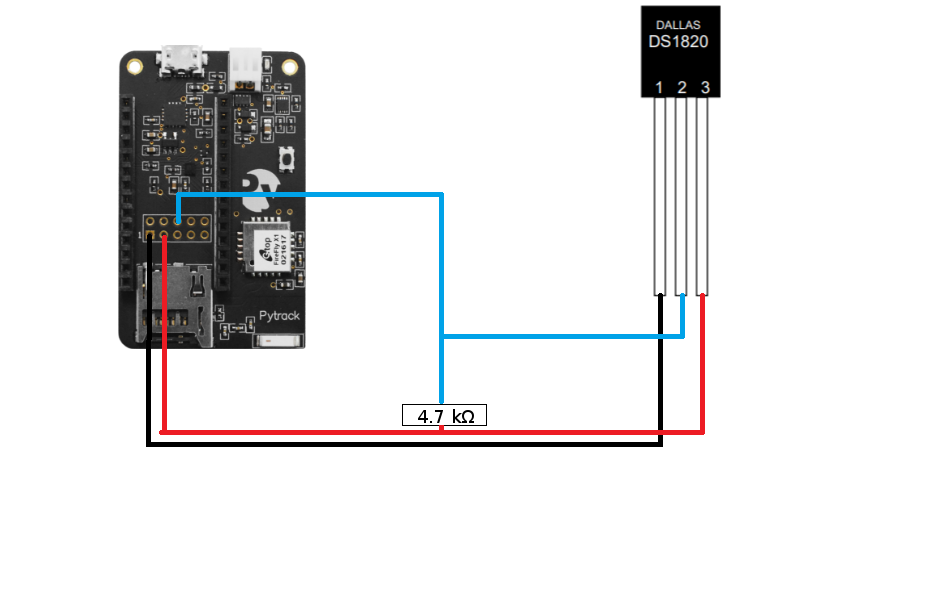
\includegraphics[width=15cm, height=9cm]{pytracktempchart}
		\end{figure}
		\begin{figure}[h]
			\caption{Temperatue sensor connection data sheet}
			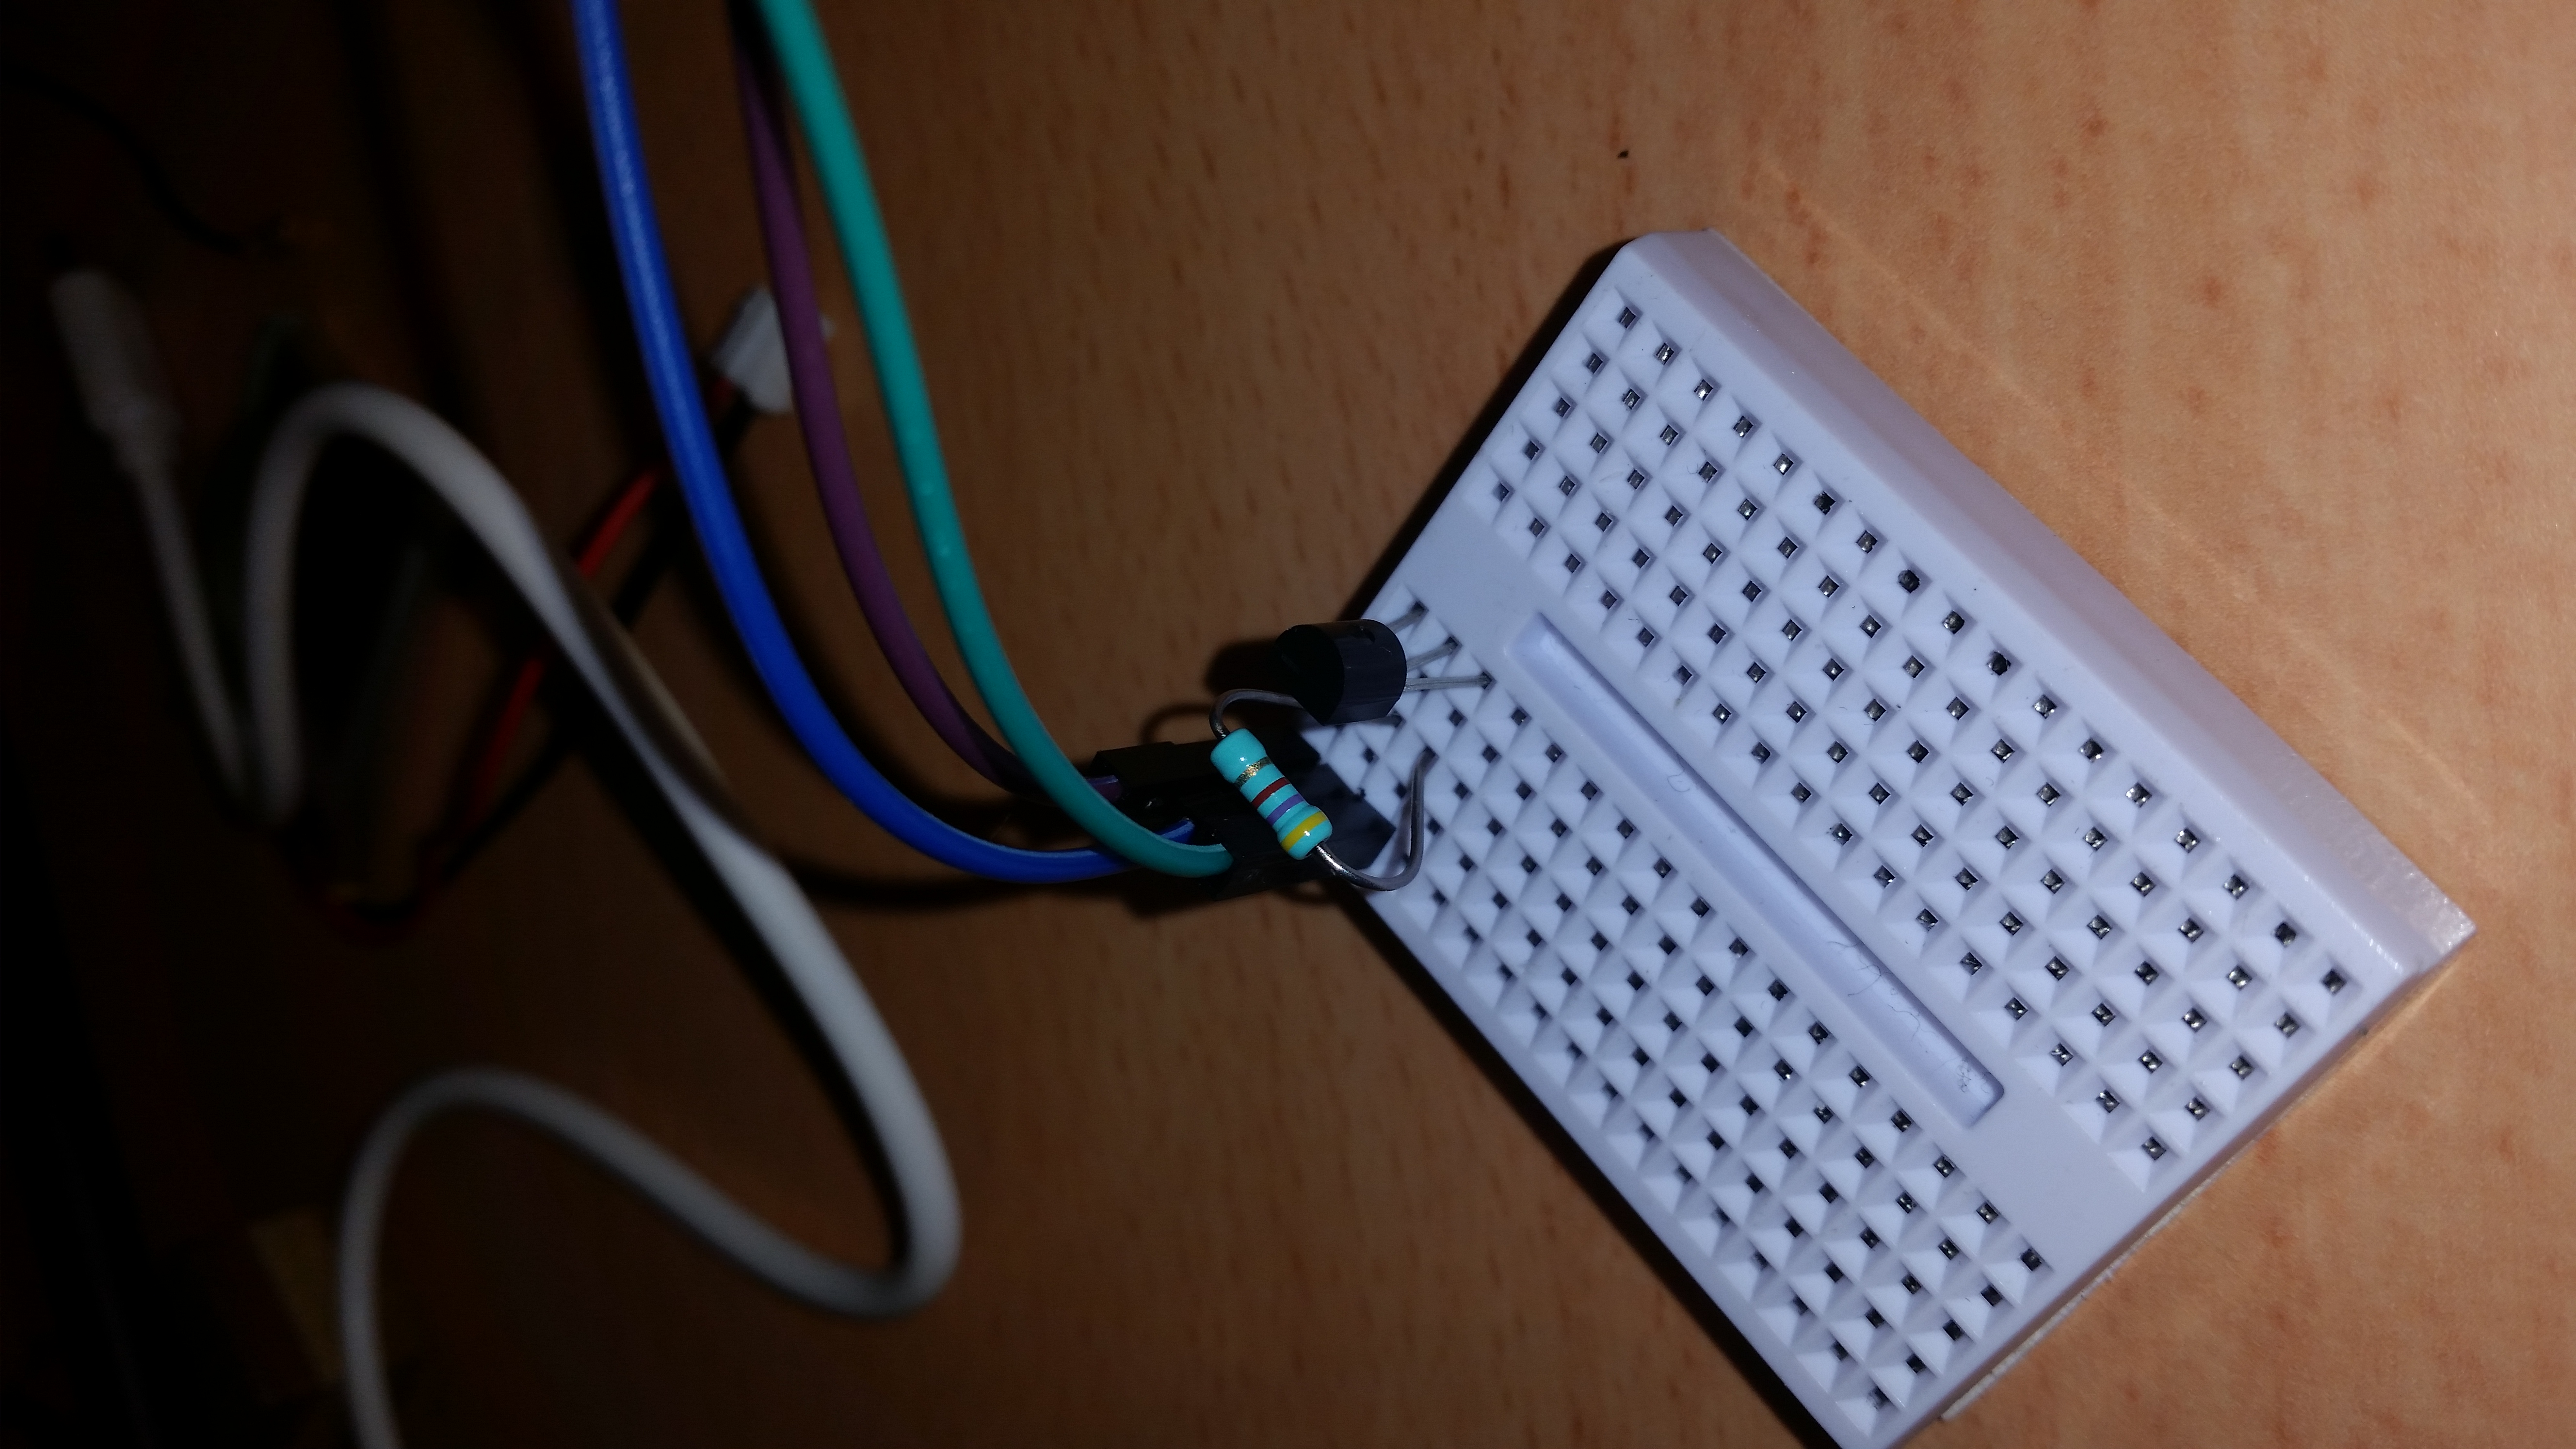
\includegraphics[width=8cm, height=8cm]{breadboard1}
		\end{figure}
		\\
		This setup proves to be successful. We observe temperature readings from the sensor at Telenor Cloud. Prior to successfully setting up the wiring, Thomas misread the datasheet once, which resulted in a temperature sensor getting destroyed. Now that we know the sensor works and the temperature readings seem to make sense, we need to attach the temperature sensor to cables. We use two stands to keep the components still while soldering. However, we realize that the Pytrack board is too thick with the cable pointing outwards from the microcontroller board. It is important to make the box as small as possible, which depends on the micro controller that is to be put inside. 
		\\\\
		We remove the connectors underneath the board and instead use connectors that are bent 90 degrees. In addition, the cables can be hidden underneath the LoPy component, decreasing the thickness even more. We solder the bent connectors to the Pytrack board. The result is displayed in figure 5. 
		\begin{figure}[h]
			\caption{Final result of Pytrack}
			\includegraphics[width=10cm, height=9cm]{pytrackendelig}
		\end{figure}
		Notice the black LoRa antenna to the right and the three temperature sensor cables to the left coming from down under the LoPy component. 
		\\\\
		The design of the box is based on being as small and lightweight as possible. Because the box is supposed to hang around an animal’s neck, the weight is in focus. It must be fairly easy to replace the battery package as well, without the risk of damaging anything. It should be waterproof as well. We use Tinkercad for designing the box. The final design is displayed in figure 6.
		\begin{figure}[h]
			\caption{The box with a Pytrack and battery package strapped onto it}
			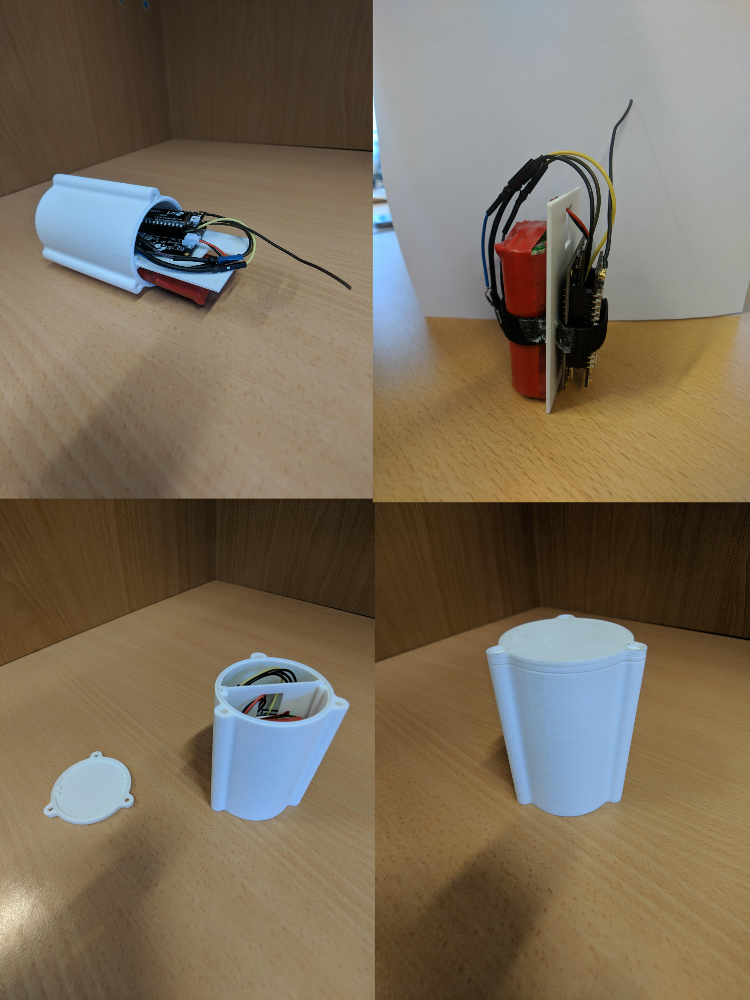
\includegraphics[width=10cm, height=13cm]{box}
		\end{figure}
		The box is split into two by a plate that can be slided in and out of it. The battery package is on one side and the Pytrack board and temperature sensor is on the other side. The battery and Pytrack are strapped to the plate with hook-and-loop fasteners. There is a hole in the plate for the battery cable. The lid has two edges for fastening the plate in it. The box was 3D printed based on the design generated in Tinkercad. In reality, we had to use the SolidWorks editor to print because we had some issues with adjusting the printer settings. All in all, the design was migrated from Tinkercad to SolidWorks.
		\\\\
		The lid is attached to the rest of the box by three screws in each hole. In addition, we 
		fill the crack in the lid with expanding foam to make the box waterproof. Furthermore, we attach the entire box around a dog’s neck to test it. We choose to use a german shepherd to test the box because of its size. For a realistic test scenario, it needs to be shaken in all directions and it needs to be pressed against the ground. The picture shows the dog wearing the tracker:
		BILDE AV LOKE
		
	\subsection{Analysis of battery consumption}
		On the edge, the battery consumption is in great focus. We send x bytes over LoRaWAN network, which is a relatively small amount of bytes, considering the fact that the LoRaWAN bandwidth is at y bytes. Taking into account that the Pytracks are in two states, namely “work” and “sleep”, we observe two different power consumption values. We use a lithium battery with 600 mAh at 3.7V. Measurements conducted when the Pytrack is in “work” state, the power consumption equals 64.4 mAh. During the “sleep” state, the consumption equals 18.2 $\mu$Ah. 
		\\\\
		We believe that it is possible to decrease the amount of data being sent. If there is not GPS coverage, “None None” is sent. We can replace that pattern with for example “N N”. Although the transmission would decrease by only 6 bytes, it is still worth pointing out this alternative. 
		\\\\
		We also want to estimate battery life of an observational unit. In this case, we use two Sony 18650 battery coupled together in parallel, delivering 3000 mAh each. Together they deliver 6000 mAh. However, they are a few years old, so the output should be somewhere below 6000 mAh.
		
\section{Conclusion}
	In this project we ventured on a task to track animals in the nature using LoRaWAN network and IoT devices. We have gained valuable insights into low-powered edge computing with limited power supply. We saw how edge computing is realized using IoT devices in a meaningful context. Looking  at the problem in question, we did solve it to a reasonable extent. Although some feature are missing, we believe we proved that the most important parts of the project were completed. At the very core, we draw a relation between the initial goal to transfer observational data over LoRaWAN and the fact that we did it. 

	\subsection{Ending state}
		

	\subsection{Relevant work}
		Rovdata uses similar tracking devices to track wolf, lynx, brown bear, wolverine and golden eagle. However, they seem to not measure temperature. Telespor is a local company based in Tromsø that provides similar services such as we do. However, they use 2G network and don't measure temperature either. 
	
	\subsection{Future work}
		An interesting aspect is any future work in the project. One of the COAT's collaboratives is interested in how positions, activity and temperature are collected. Those three data points can be correlated to each other to see the relation between changes. For example, in one season the temperature is at $a$ degrees Celsius in a particular area. Furthermore, there are $x$ individuals in this area. The next year, there can be a lower temperature in the same area. At the same time, it is counted less than $x$ individuals of the same species. By looking at correlation, one can predict migration patterns, given temperature fluctuations. In fact, Thomas has been in dialog with one of the COAT collaborators about a potential Master's Thesis that builds upon some aspects of this project. 
		\\\\
		For a real-world application, the box's mass should be decreased. It's somewhat heavy, even for a 50 kg fully-grown German shepherd. As of now, we are able to track animals of similar size, but not smaller-sized animals. 
		
	
		

\begin{thebibliography}{9}
	\bibitem{tempsensor}
	\textit{DS18B20 data sheet}
	\\\texttt {https://datasheets.maximintegrated.com/en/ds/DS18B20.pdf}
	
	\bibitem{LoRaWAN}
	\textit{LoRaWAN overview}
	\\\texttt {https://www.thethingsnetwork.org/docs/lorawan/, 2018}
	
	\bibitem{wikiMQTT}
	\textit{MQTT overview}
	\\\texttt {https://en.wikipedia.org/wiki/MQTT, 2018}
	
	\bibitem{telenorIOT}
	\textit{Telenor Managed IoT Cloud}
	\\\texttt{https://startiot.telenor.com/lessons/mqtt-and-managed-iot-cloud/, 2018}
	
	
\end{thebibliography}


\end{document}



